\documentclass{report}



\usepackage{amsmath}
\usepackage{graphics}
\usepackage{textcomp}


%---Scale Command----%

\newcommand\scalemath[2]{\scalebox{#1}{\mbox{\ensuremath{\displaystyle #2}}}}

\input{preamble}
\input{macros}
\input{letterfonts}

\pagenumbering{arabic}

\title{\Huge{Applied Logic}\\Modal Logic}
\author{\huge{Jacek Grzegorzewski}}
\date{}

\begin{document}
\maketitle
\newpage% or \cleardoublepage
% \pdfbookmark[<level>]{<title>}{<dest>}
\pdfbookmark[section]{\contentsname}{toc}
\tableofcontents
\pagebreak

\dfn{Kripke's frame}{A Kripke's frame is $(X,R)$ where $R \subset X \times X$}
\dfn{Valuation}{$\pi:P  \longrightarrow P(x) $ is a valuation}

\dfn{Kripke's model}{A Kripke's model is $(X,R,\pi) = \mathbb{M}$}

\dfn{Semantics}{Semantics having $\phi \in \mathcal{L}_{ML}(\mathbb{P})$ and $\mathcal{M}$ and  $x \in X$,  $\mathbb{M}, x \vdash \phi$
	\begin{itemize}
		\item $\mathbb{M}{x} \vdash p \equiv x \in \pi(p)$
		\item $\mathbb{M}{x} \vdash \phi \vee \psi \equiv \mathbb{M}{x} \vdash \phi \vee \mathbb{M}{x} \vdash \psi$
		\item $\mathbb{M},x \vdash \neg \phi \equiv \neg \mathbb{M},x  \vdash \phi $
		\item $\mathbb{M},x \vdash \square \phi \equiv \forall y \in X ((x,y) \in R \rightarrow \mathbb{M},x \vdash \phi )$
		\item $\mathbb{M},x \vdash \diamond\phi \equiv \exists y \in X ((x,y) \in R \wedge \mathbb{M},y \vdash \phi ) $
	\end{itemize}
	
}





\ex{Simple world}{Let:\\ \begin{itemize}
		\item $\mathcal{P} = \{ p, q\}$ 
		\item $X = \{a, b, c\}$
		\item  $R = \{(b,a), (b,c), (c,c)\}$
		\item  $\pi(p) = \{a, b, c\}$
		\item $\pi(q) = \{b, c\}$
	\end{itemize}
	The following statements are then true:
	\begin{itemize}
		\item $\mathbb{M},a \vdash p $ 
		\item $ \mathbb{M},a \vdash \square p$
		\item $\mathbb{M},a \vdash \neg \diamond q  $
	\end{itemize} 
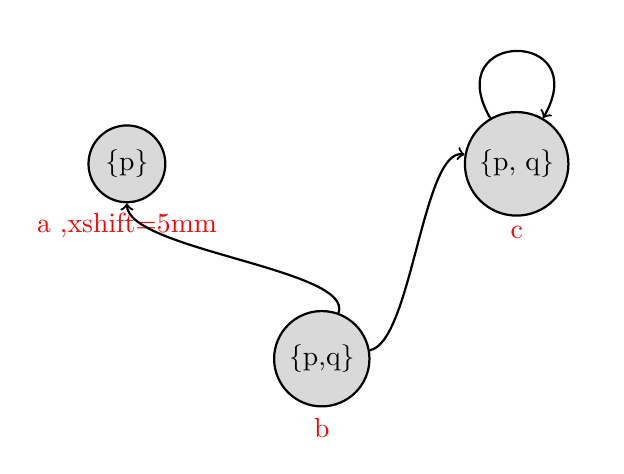
\begin{tikzpicture}[thick,node distance = {35mm},  main/.style = {draw, circle}]
	\node[main, fill = gray!30, label={[red]below:b}](1) {\{p,q\}};
	\node[main, fill = gray!30, label={[red]below:a ,xshift=5mm}] (2) [above left of=1] {\{p\}};
	\node[main, fill = gray!30, label={[red]below:c}] (3) [above right of=1] {\{p, q\}};
	\draw[->] (1) to [out=70, in=270, looseness=0.5] (2);
	\draw[->] (1) to [out=10, in=170, looseness=0.5] (3);
	\draw[->] (3) to [out=120, in=60, looseness=5] (3);
	
	\end{tikzpicture}
	}


	



	

\end{document}
